\subsection{Bipolar transistors}
A byproduct of the Bulk CMOS structure is a pair of parasitic bipolar transistors.\footnote{\url{http://www.analog.com/en/analog-dialogue/articles/winning-the-battle-against-latchup.html}}
The collector of each BJT is connected to the base of the other transistor in a positive feedback structure.
A phenomenon called latchup can occur when both BJT's conduct, creating a low resistance path between VDD and GND and the product of the gains of the two transistors in the feedback loop $\beta_1 \times \beta_2$ is greater than one.
The result of latchup is at the minimum a circuit malfunction, and in the worst case, the destruction of the device.

\begin{figure}[H]
	\centering
	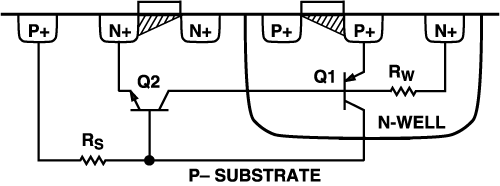
\includegraphics[scale=0.5]{latchup_cross.png}
	\caption{Lateral and vertical parasitic BJT}
	\label{latchup_diagram}
\end{figure}

In \autoref{latchup_diagram} we can see the two above mentioned transistors. In order to find out their average $\beta$ we split it up into two separate test circuits, allowing us to measure their properties out with probes on our test wafer.

\subsubsection{Lateral bipolar transistor}


\subsubsection{Vertical bipolar transistor}